\documentclass[11pt,letterpaper]{article}
\usepackage[margin=0.78in]{geometry}
\usepackage[T1]{fontenc}
\usepackage{graphicx}
\usepackage{booktabs}
\usepackage{array}
\usepackage[colorlinks=true,urlcolor=blue,linkcolor=blue]{hyperref}
\setlength{\parskip}{0.38em}
\setlength{\parindent}{0pt}
\emergencystretch=2em
\urlstyle{same}

\title{CS 422 Assignment 3: Adaptive Delay/Loss AIMD\\Option 1 --- Linux TCP Congestion-Control Module}
\author{CS 422 project team}
\date{October 2026}

\begin{document}
\maketitle

\begin{abstract}
We implemented a Linux TCP congestion-control module, \texttt{cs422\_custom},
and compared it with CUBIC, Reno, and BBR on ten public iperf3 destinations.
Each algorithm was scheduled for three 10-second runs per destination with
one-second TCP\_INFO sampling. Of 120 selected tests, 119 succeeded; the only
failure was a Reno timeout. The custom algorithm averaged 56.6 Mbps acknowledged
goodput and 158.9 ms RTT across its 30 successful runs. BBR achieved higher
goodput (78.4 Mbps) but also higher RTT (168.2 ms) and more retransmissions.
These are descriptive Internet-path results, not proof of universal superiority.
\end{abstract}

\section{Submission and code map}
Repository: \href{https://github.com/RohMalpani/NetworksAssignment1/tree/main/assignment3}{Assignment 3 folder on GitHub}.
The source map below links directly to the relevant functions:
\begin{itemize}
\item Controller callbacks:
\href{https://github.com/RohMalpani/NetworksAssignment1/blob/main/assignment3/kernel/tcp_cs422.c\#L47-L230}{\texttt{tcp\_cs422.c}, lines 47--230}.
\item Data-socket selection and read-back:
\href{https://github.com/RohMalpani/NetworksAssignment1/blob/main/assignment3/client/iperf3_client.py\#L91-L140}{\texttt{iperf3\_client.py}, lines 91--140}.
\item TCP sampling and goodput:
\href{https://github.com/RohMalpani/NetworksAssignment1/blob/main/assignment3/client/goodput.py\#L32-L87}{\texttt{goodput.py}, lines 32--87}.
\item Experiment scheduling:
\href{https://github.com/RohMalpani/NetworksAssignment1/blob/main/assignment3/run_experiments.py\#L53-L149}{\texttt{run\_experiments.py}, lines 53--149}.
\item Audit and figures:
\href{https://github.com/RohMalpani/NetworksAssignment1/blob/main/assignment3/plot_results.py\#L51-L258}{\texttt{plot\_results.py}, lines 51--258}.
\end{itemize}
The repository contains the raw CSVs, configuration, run log, module source,
plotting code, and the final PDF.

\section{Controller design and implementation}
Our Adaptive Delay/Loss AIMD controller keeps the Linux TCP congestion window
(\texttt{snd\_cwnd}) in segments. It leaves TCP's initial window and slow-start
threshold unchanged. Its private state starts with unknown minimum RTT and
delivery rate, zero counters, and an armed delay-reduction flag. The code uses
the following signals: ACK-derived delivered packets per second from
\texttt{tp->delivered}, smoothed RTT from \texttt{tp->srtt\_us}, a ten-second
minimum-RTT window, and kernel loss/recovery callbacks. The estimated queue
ratio is $(\mathrm{SRTT}-\mathrm{minRTT})/\mathrm{minRTT}$, clamped conceptually at
zero. An unavailable RTT or rate falls back to Reno-like additive growth.

At most once per smoothed RTT, a congestion-window-limited round contributes a
delivery-rate sample to an EWMA with weight $1/4$ on the new sample. After at
least three valid rounds, two rounds with queue ratio at least 20\% or with
rate growth at most 5\% can end slow start. In congestion avoidance, growth is
about one segment per RTT; it becomes about two only below 10\% queueing when
delivery improves by more than 3\%. Growth is held above 20\% queueing. Two
high-delay rounds with growth below 3\% can trigger a one-time 10\% window
reduction, followed by a one-round cooldown; the mechanism rearms after the
queue estimate falls below 10\%.

On a loss event, \texttt{ssthresh} is ordinarily half the current window.
When delay is low, delivery has fallen by less than 10\%, and there is no
timeout evidence, the threshold is instead 85\% of the window. TCP's own
recovery machinery handles retransmission and the subsequent window reduction.
The module registers with \texttt{tcp\_congestion\_ops} and does not replace
the TCP stack. Relative to the Assignment 2 pseudocode, the implementation
explicitly clears stale delivery-growth evidence after a non-window-limited
round rather than merely skipping one update. Its thresholds are hypotheses,
not parameters fitted to this test data.

\section{Measured Linux environment and build}
The saved \path{results/run_config.json} reports the exact measured kernel:
\begin{center}\texttt{6.6.87.2-microsoft-standard-WSL2}\end{center}
The module must be built for that running kernel's release, configuration,
symbol versions, and architecture;
an Ubuntu header package for another kernel is not interchangeable. Required
capabilities are loadable modules (\texttt{CONFIG\_MODULES}), the Linux TCP
congestion-control API and TCP\_INFO, and selectable CUBIC, Reno, and BBR.
The measured WSL2 setup used \texttt{CONFIG\_MODVERSIONS=y}; therefore a
matching \texttt{Module.symvers} is required. The build commands use
\texttt{/proc/config.gz} (requiring \texttt{CONFIG\_IKCONFIG\_PROC}) to copy
the running configuration. The kernel source is Microsoft's
\path{linux-msft-wsl-6.6.87.2} tag, not generic upstream Linux.

The build and load sequence below is for the measured WSL2 kernel. It requires
\texttt{build-essential}, \texttt{flex}, \texttt{bison}, \texttt{libssl-dev},
\texttt{libelf-dev}, \texttt{bc}, \texttt{dwarves}, \texttt{git}, and Python 3.
The source clone is disposable; moving its \texttt{.git} directory aside avoids
an unwanted \texttt{+} suffix in the module's kernel release. A full
\texttt{make modules}, rather than only \texttt{modules\_prepare}, generates
the needed \texttt{Module.symvers} for versioned symbols.

\begin{verbatim}
uname -r  # must print 6.6.87.2-microsoft-standard-WSL2
sudo apt update
sudo apt install -y build-essential flex bison libssl-dev libelf-dev \
  bc dwarves git python3 python3-venv
git clone --depth 1 -b linux-msft-wsl-6.6.87.2 \
  https://github.com/microsoft/WSL2-Linux-Kernel.git ~/WSL2-Linux-Kernel
cd ~/WSL2-Linux-Kernel
zcat /proc/config.gz > .config
make olddefconfig
mv .git .git.saved
make -j"$(nproc)" modules
cd <repo>/assignment3/kernel
make KDIR=~/WSL2-Linux-Kernel
modinfo -F vermagic tcp_cs422.ko
sudo modprobe tcp_bbr
sudo insmod tcp_cs422.ko
cat /proc/sys/net/ipv4/tcp_available_congestion_control
\end{verbatim}

\texttt{modinfo} must show a vermagic release beginning with the exact
\texttt{uname -r}; the available-algorithm list must contain
\texttt{cs422\_custom}, \texttt{cubic}, \texttt{reno}, and \texttt{bbr}. The group's
WSL2 setup notes record a successful compile, load, and socket-selection
check. No compiler or \texttt{insmod} transcript was retained in the submitted
raw files; therefore the required live grading demonstration remains necessary.
The 30 successful \texttt{cs422\_custom} transfers, with the data socket's
\texttt{TCP\_CONGESTION} read-back stored in the run records, provide runtime
evidence for the measured session. They do not independently establish the
identity of the compiled binary. WSL restarts unload the module; reload it
before a demonstration. Remove it after its sockets close with
\texttt{sudo rmmod tcp\_cs422}. The global default TCP algorithm is not changed.

The external-module build procedure follows the
\href{https://docs.kernel.org/kbuild/modules.html}{Linux kernel kbuild documentation};
the tagged source comes from
\href{https://github.com/microsoft/WSL2-Linux-Kernel}{Microsoft's WSL2 kernel repository}.

\section{Matched experiment and measurements}
The run used ten accepted destinations, three repetitions, four algorithms,
ten seconds per transfer, a nominal one-second sampling interval, a three-second
pause between tests, seed 422, and a maximum of ten rejected candidates. The
order was cyclically rotated by destination index and repetition, so no
algorithm always ran first. The same accepted host and port were reused for
all four algorithms and all repetitions. Repetition 1 accepted a destination
only if all four tests succeeded; three failed candidates were replaced.
\texttt{results/run\_config.json} records the parameters and accepted pairs;
\texttt{results/runs.csv} records every attempt, outcome, error, sequence number,
and order position; \texttt{results/run\_log.txt} preserves console output.

Before connecting the data socket, the client calls
\texttt{setsockopt(TCP\_CONGESTION)} for the requested algorithm. After connecting,
it reads \texttt{getsockopt(TCP\_CONGESTION)} and stores the algorithm actually
used in \texttt{runs.csv}. The separate control socket does not carry the bulk
measurement. Every sampling interval, \texttt{getsockopt(TCP\_INFO)} on the data
socket supplies \texttt{snd\_cwnd} (segments), RTT (microseconds), cumulative
retransmissions, and acknowledged bytes. Interval goodput is
$8\Delta\mathrm{bytes\_acked}/\Delta t$, reported in Mbps. The loss signal is
the nonnegative increment of cumulative retransmissions per interval; it is
a proxy, not a direct count of all drops or duplicate ACKs.

Our audit of the saved files found 132 raw attempts: 12 tests on rejected
candidates and 120 planned tests on the ten accepted destinations. Of the
latter, 119 succeeded; Reno timed out on Copenhagen in repetition 3. All 119
successful selected tests have TCP\_INFO samples, and no selected run key is
missing or duplicated. The saved algorithm and order position match the
requested cyclic order. The selected tests contain 1,161 samples. Seven
successful traces have fewer than the expected ten samples, mostly on the
Copenhagen path, because sampling occurs after a blocking data send returns.
They remain in the raw files and the main descriptive analysis; the sensitivity
check below excludes them. A successful protocol exchange alone does not
guarantee ten evenly spaced samples.

\section{Results and interpretation}
For each successful run, we take the arithmetic mean of its observed interval
goodputs and RTTs, then summarize those per-run means. Retransmissions are
summed within each run. Rejected candidate servers and the failed Reno test
are excluded from aggregate values. Standard deviations below describe
cross-run variability, not confidence intervals.

\begin{center}
\small
\begin{tabular}{lrrrrrr}
\toprule
Algorithm & $n$ & Goodput mean & Goodput median & Goodput SD & RTT mean & RTT median \\
 & & Mbps & Mbps & Mbps & ms & ms \\
\midrule
CUBIC & 30 & 43.7 & 30.8 & 40.4 & 162.6 & 128.0 \\
Reno & 29 & 54.4 & 31.4 & 49.3 & 163.1 & 136.7 \\
BBR & 30 & 78.4 & 76.1 & 44.3 & 168.2 & 139.1 \\
Custom & 30 & 56.6 & 38.8 & 48.8 & 158.9 & 129.1 \\
\bottomrule
\end{tabular}
\end{center}
\vspace{-0.4em}
\begin{center}\small Table 1: Per-run aggregate goodput and RTT across selected destinations.
Mean retransmissions per successful run were 241.9 (CUBIC), 315.3 (Reno),
2,556.5 (BBR), and 353.7 (custom).\end{center}

\begin{figure}[h]
\centering
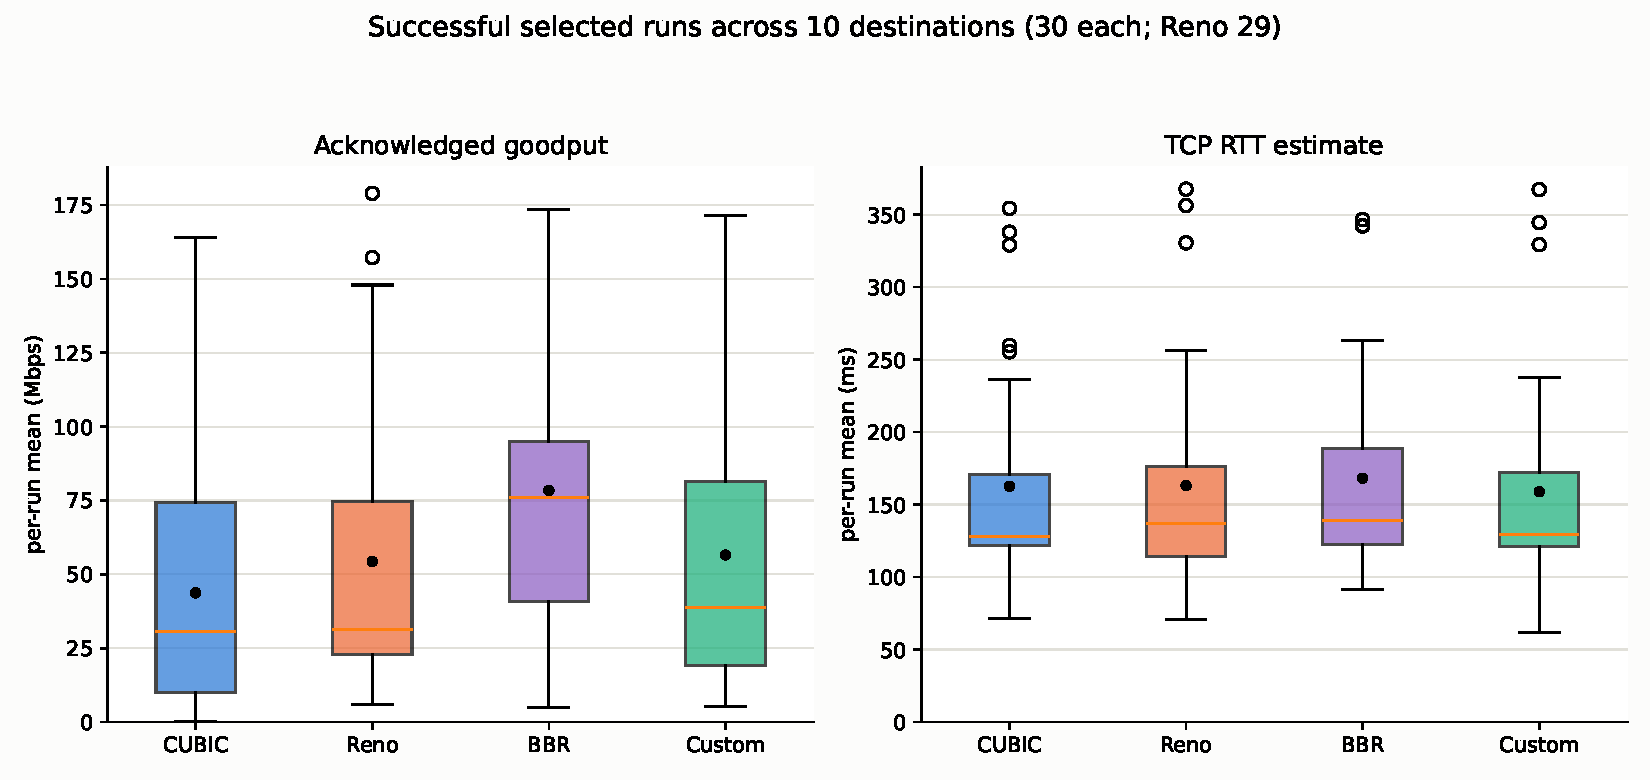
\includegraphics[width=\textwidth]{plots/aggregate_distributions.pdf}
\caption{Per-run goodput and RTT distributions. Black dots mark arithmetic
means; boxes show medians and interquartile ranges. The one failed Reno run
is excluded, and destination effects are not controlled in these boxes.}
\end{figure}

The custom controller's average goodput exceeded CUBIC by 12.8 Mbps and Reno
by 2.2 Mbps, but trailed BBR by 21.9 Mbps in the unequal-success aggregate.
Its average RTT was 9.3 ms lower than BBR's. Restricting to the 29 complete
destination--repetition groups containing all four successful tests gives
paired mean custom-minus-baseline goodput differences of $+14.2$ Mbps versus
CUBIC, $+3.9$ versus Reno, and $-17.4$ versus BBR. On these matched groups,
the custom controller's average RTT was 9.8 ms lower than BBR's. This supports
a throughput--RTT tradeoff relative to BBR, not an across-the-board performance
improvement. BBR also showed far more retransmissions, but retransmission
counts are path- and load-sensitive and should not be equated directly to
packets lost in the network.

\begin{center}
\small
\begin{tabular}{lrrrr}
\toprule
Destination & CUBIC & Reno & BBR & Custom \\
\midrule
Milan & 86.9 & 115.4 & 111.5 & 120.3 \\
Madrid & 90.9 & 99.7 & 68.4 & 115.8 \\
Luanda & 71.8 & 60.5 & 67.3 & 56.0 \\
Paris & 36.4 & 62.9 & 89.7 & 48.7 \\
Santa Ana & 5.0 & 24.1 & 83.6 & 32.5 \\
Fuzhou & 17.7 & 30.8 & 52.2 & 49.0 \\
Los Angeles & 77.4 & 87.8 & 134.3 & 80.7 \\
Nairobi & 13.0 & 14.5 & 35.8 & 30.9 \\
Alvsjo & 21.2 & 24.4 & 31.5 & 24.7 \\
Copenhagen & 17.2 & 8.1\textsuperscript{*} & 110.3 & 7.1 \\
\bottomrule
\end{tabular}
\end{center}
\vspace{-0.4em}
\begin{center}\small Table 2: Mean of successful per-run goodputs (Mbps) by
destination. \textsuperscript{*}Copenhagen Reno uses two successful runs;
its third timed out.\end{center}

BBR had the highest destination-average goodput on seven paths, custom on
two (Milan and Madrid), and CUBIC on one (Luanda). The rankings changed
substantially between repetitions. On the Paris representative path, custom
goodput fell from 95.4 to 44.8 to 5.9 Mbps across the three repetitions,
while BBR delivered 115.0, 75.1, and 79.0 Mbps. This variability prevents a
strong causal or statistical claim from three public-server runs. The WSL2
network path, server load, cross traffic, and sequential rather than simultaneous
tests are possible confounders. The short-trace sensitivity check retains the
ranking: when only ten-sample successful runs are kept, mean goodputs are
46.5 (CUBIC, $n=28$), 57.8 (Reno, $n=27$), 81.0 (BBR, $n=29$), and
60.1 Mbps (custom, $n=28$).

\section{Representative-destination visualizations}
The plotting code chooses the accepted destination closest to the median of
pooled destination mean goodputs, among paths with complete, fully sampled
four-algorithm traces. This selects \texttt{96.45.42.156:30004} (Paris), for
which all twelve tests have ten samples. Every panel below uses that same
host/port and the same axis limits across the four algorithms. Blue, orange,
and green denote repetitions 1, 2, and 3. Pages 1--4 repeat the required
time-series plots; pages 5--7 repeat the goodput scatter plots from Assignment 2
Question 2(b). The loss axis is retransmissions per interval, not a direct
packet-drop count.

\clearpage
\subsection*{1. Congestion window over time}
\begin{center}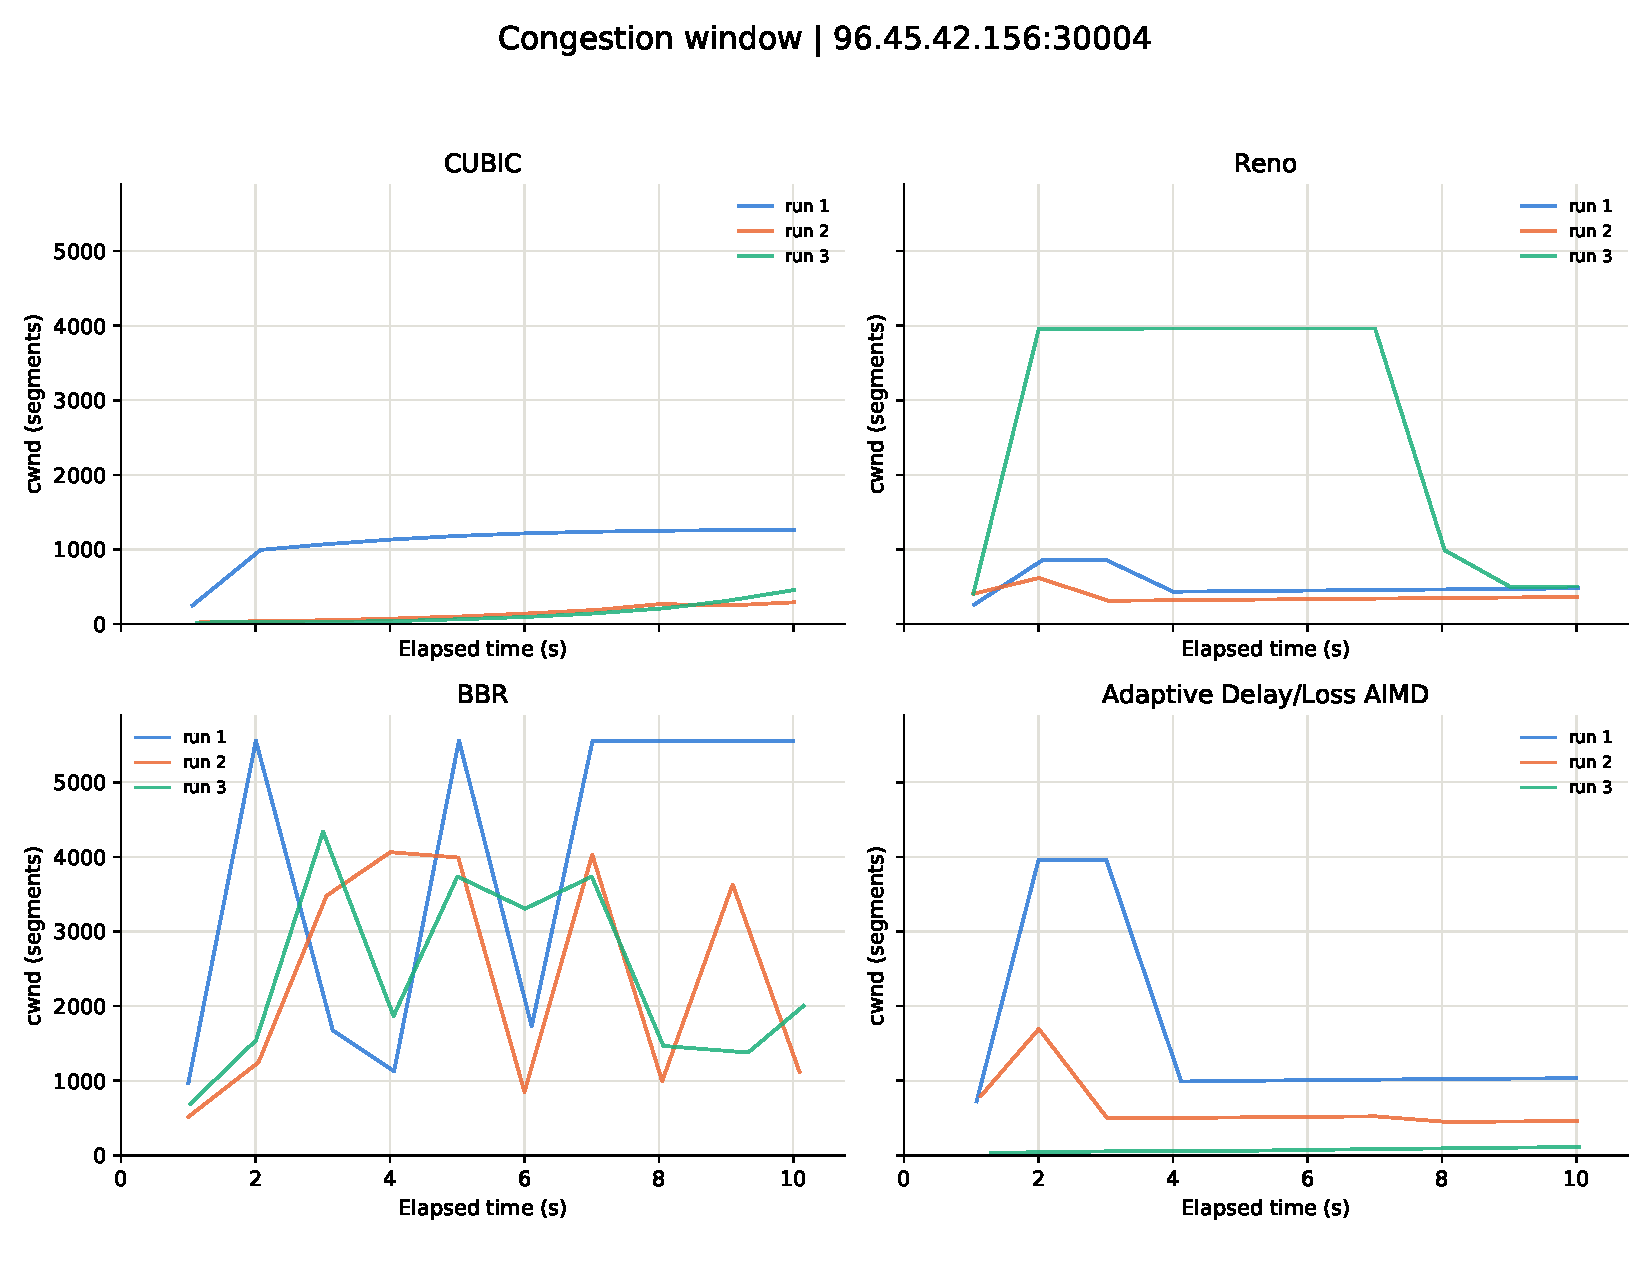
\includegraphics[page=1,width=\textwidth]{plots/option1_comparison.pdf}\end{center}
On this Paris path, BBR maintained the largest mean congestion window
(2,895 segments), followed by Reno (1,169), custom (762), and CUBIC (457).
The custom third run stayed between 35 and 112 segments and delivered only
5.8 Mbps; its first run peaked at 3,963 segments and averaged 95.4 Mbps.
Reno also briefly reached 3,962 segments in its third run. These are
kernel-reported \texttt{snd\_cwnd} values, not bytes, and their variation
between runs cautions against treating one window trace as typical.

\clearpage
\subsection*{2. RTT over time}
\begin{center}\includegraphics[page=2,width=\textwidth]{plots/option1_comparison.pdf}\end{center}
Mean sampled RTT on Paris was 134.0 ms for custom, 139.6 for Reno, 143.5
for CUBIC, and 148.5 for BBR. BBR's third run averaged 159.0 ms, whereas
custom's third run averaged 127.7 ms. Yet that custom run had the lowest
goodput of its three repetitions. Lower RTT here therefore did not
necessarily mean higher delivery rate; path conditions and run order could
also affect the observed delay.

\clearpage
\subsection*{3. Retransmission proxy over time}
\begin{center}\includegraphics[page=3,width=\textwidth]{plots/option1_comparison.pdf}\end{center}
BBR recorded 7,886 retransmissions across its three Paris traces, versus
961 for custom, 960 for CUBIC, and 901 for Reno. BBR had a nonzero
retransmission increment in 23 of 30 intervals, while the other algorithms
had only three to six such intervals each. Its third run included the
largest burst (1,175). This is a TCP retransmission proxy, not a count of
all path drops, and the plot cannot identify where losses occurred.

\clearpage
\subsection*{4. Acknowledged goodput over time}
\begin{center}\includegraphics[page=4,width=\textwidth]{plots/option1_comparison.pdf}\end{center}
BBR sustained the highest mean interval goodput on Paris (89.7 Mbps), with
its three run means between 75.0 and 115.0 Mbps. Reno averaged 62.9 Mbps
but ranged from 28.6 to 115.9 across runs. Custom averaged 48.7 Mbps,
falling from 95.4 in run 1 to 5.8 in run 3; CUBIC averaged 36.3 Mbps and
also had two runs near 10 Mbps. The run-to-run spread is large enough that
a single trace would give a misleading ranking.

\clearpage
\subsection*{5. Goodput versus congestion window}
\begin{center}\includegraphics[page=5,width=\textwidth]{plots/option1_comparison.pdf}\end{center}
The CUBIC and Reno points generally move upward as their reported
congestion windows grow; their high-throughput runs also occupy the
right-hand side of their panels. BBR's points extend farther right because
its mean window is 2,895 segments, yet goodput varies even at large
windows. Custom's low-throughput third run clusters at small windows.
Each point is one interval, but pooling three sequential runs can make
between-run differences look like a within-run causal relationship.

\clearpage
\subsection*{6. Goodput versus RTT}
\begin{center}\includegraphics[page=6,width=\textwidth]{plots/option1_comparison.pdf}\end{center}
There is no consistent lower-RTT/higher-goodput pattern across the four
panels. BBR delivered 89.7 Mbps on average despite the highest mean RTT
(148.5 ms); custom had the lowest mean RTT (134.0 ms) but only 48.7 Mbps.
In particular, custom's low-goodput third run averaged 127.7 ms RTT.
The shared scales show substantial overlap in RTT while goodput differs,
so RTT alone does not explain the throughput ranking.

\clearpage
\subsection*{7. Goodput versus retransmission proxy}
\begin{center}\includegraphics[page=7,width=\textwidth]{plots/option1_comparison.pdf}\end{center}
Many intervals have zero new retransmissions but widely different
goodputs, so absence of a retransmission event does not predict high
throughput. BBR also maintained high goodput while recording the most
retransmissions overall (7,886 across three runs). The shared horizontal
scale accommodates its 1,175-event burst and compresses the near-zero
points in the other panels. These points show coexistence, not that
retransmissions improved throughput or that every retransmission followed
network congestion.

\clearpage
\section{Reproduction, provenance, and grading demonstration}
From \texttt{assignment3/} on the compatible WSL2 host, first build and load
the module as above. Then reproduce the matched experiment without replacing
the committed raw files:
\begin{verbatim}
python3 -m venv .venv
. .venv/bin/activate
python3 -m pip install -r requirements.txt
python3 run_experiments.py --servers servers.csv -n 10 --duration 10 \
  --interval 1 --reps 3 --algorithms cubic reno bbr cs422_custom \
  --pause 3 --max-failures 10 --seed 422 \
  --out-dir results/reproduction
python3 plot_results.py --results-dir results/reproduction \
  --plots-dir plots/reproduction
\end{verbatim}
The Python client itself uses the standard library; Matplotlib is required
only for offline plotting. \path{results/runs.csv} is one row per attempt,
including failed and rejected candidates. \path{results/samples.csv} is one
row per observed interval. \path{results/run_config.json} records the run ID,
kernel release, destination pairs, test parameters, and seed.
\path{results/run_log.txt} gives the rotation and failure messages.
\path{results/analysis_summary.json} records the audit counts, representative
selection, aggregation method, and computed statistics. The plots can be
regenerated from the committed raw files with \path{python3 plot_results.py}
on any machine with Python and Matplotlib; no network test or kernel module is
needed for that step.
Regenerating this PDF requires Tectonic 0.17 or a \LaTeX{} distribution with
\texttt{geometry}, \texttt{graphicx}, \texttt{booktabs}, and \texttt{hyperref};
run \texttt{tectonic report.tex} after generating the plot PDFs.

During grading, the team should show \texttt{uname -r}, rebuild against that
exact kernel, inspect \texttt{modinfo -F vermagic}, load the module, check that
\texttt{cs422\_custom} appears in the available-algorithm list, and demonstrate
that a Python TCP socket accepts and reads back
\texttt{TCP\_CONGESTION=cs422\_custom}. A short live iperf3 transfer can then
show \texttt{TCP\_INFO} samples. The grading environment itself is not expected
to load the module. If the grading machine's kernel differs from
\texttt{6.6.87.2-microsoft-standard-WSL2}, rebuild with its own matching
sources/configuration before the demonstration.

\section{AI use}
AI tools assisted with the original pseudocode and module draft, the WSL2
build setup, CSV auditing, plotting code, and report drafting. Design decisions
and AI usage are documented in \texttt{DECISIONS.md} and \texttt{AI\_USAGE.md}.

\end{document}
